% LaTeX source for ``การเรียนรู้ของเครื่องสำหรับเคมีควอนตัม (Machine Learning for Quantum Chemistry)''
% Copyright (c) 2022 รังสิมันต์ เกษแก้ว (Rangsiman Ketkaew).

% License: Creative Commons Attribution-NonCommercial-NoDerivatives 4.0 International (CC BY-NC-ND 4.0)
% https://creativecommons.org/licenses/by-nc-nd/4.0/

\chapter{การเรียนรู้แบบมีผู้สอน}
\label{ch:sup_ml}

\begin{figure}[htbp]
    \centering
    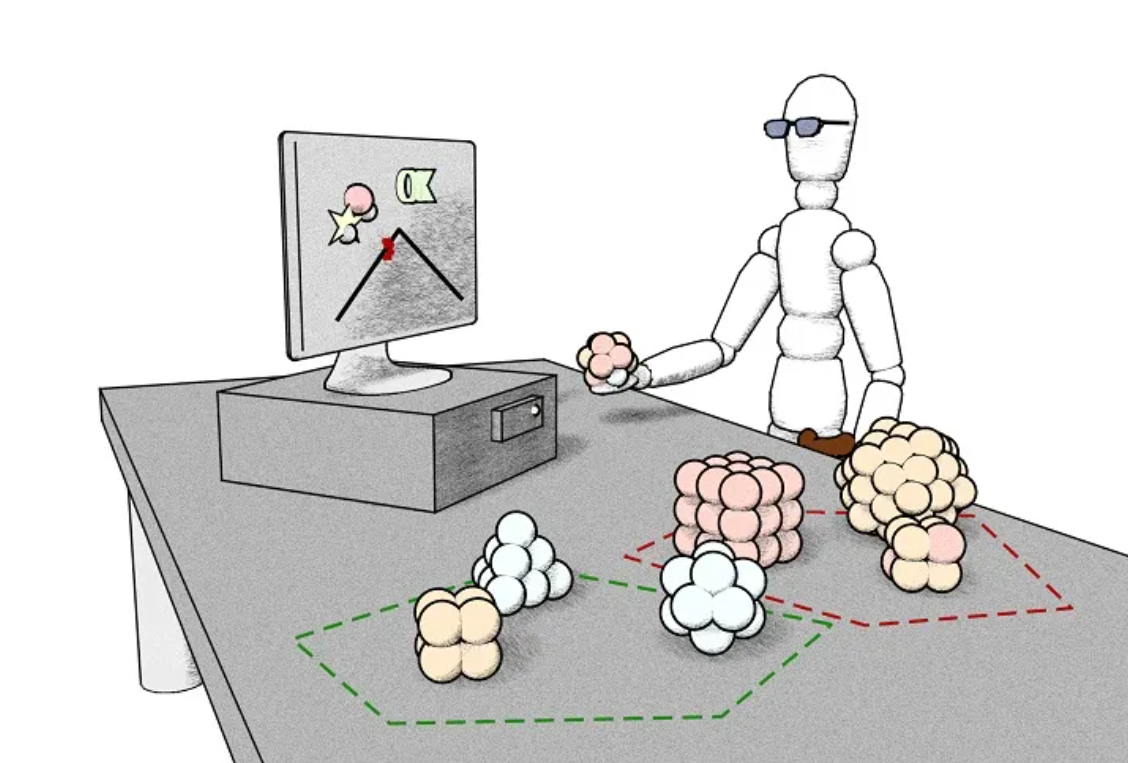
\includegraphics[width=0.9\linewidth]{fig/supervised_ml.png}
    \caption{หุ่นยนต์กำลังเรียนรู้หาความเชื่อมโยงระหว่างโครงสร้างกับคุณสมบัติของโมเลกุล (เครดิตภาพ: https://puentesdigitales.com)}
    \label{fig:supervised_ml}
\end{figure}

การเรียนรู้แบบมีผู้สอนหรือ Supervised Learning เป็นเทคนิคแรก ๆ ที่ถูกพัฒนาขึ้นมาในช่วงยุคเริ่มต้นของ ML ซึ่งเป็นแนวคิดที่ใช้อินพุตและ%
เอาต์พุตในการฝึกสอนโมเดล ซึ่งโมเดลที่ได้ออกมานั้นจะเก็บข้อมูลที่อธิบายความสัมพันธ์ระหว่างอินพุตและเอาต์พุตนั่นเอง $($เปรียบเสมือนฟังก์ชัน%
ทางคณิคศาสตร์ $f(x))$ ซึ่งผู้เขียนมีความคิดเห็นส่วนตัวว่าการสร้างโมเดลประเภทนี้ง่ายกว่าประเภทอื่นทั้งในแง่ทฤษฎีของอัลกอริทึม การเรียนรู้ของ%
ผู้เริ่มต้นศึกษาและการนำไปใช้จริง โดยเทคนิคนี้ได้รับความนิยมมากที่สุดนั่นก็เพราะว่าสามารถนำไปประยุกต์ใช้งานกับโจทย์ที่หลากหลาย

Supervised ML เป็นเทคนิคที่เข้าใจได้ง่ายที่สุดเพราะว่าเป็นการฝึกให้โมเดลมีความสามารถในการเรียนรู้ Target อย่างตรงไปตรงมา จริง ๆ นิยาม%
ของ Supervised ML นั้นมีหลายนิยามมาก ขึ้นอยู่กับว่าเราต้องการนิยามในเชิงปรัชญา เชิงคณิตศาสตร์ หรือเชิงปฏิบัติ ทุกครั้งที่มีคนถามผู้เขียนว่า 
Supervised ML คืออะไร ผู้เขียนก็มักจะตอบไปสั้น ๆ ว่า \enquote{\textit{Supervised ML (จริง ๆ แล้ว ML ทุกอัลกอริทึมเลยก็ว่า) 
คือการ Fit Curve}} ซึ่งการให้นิยามแบบนี้เป็นในเชิงปฏิบัติ ตัวอย่างเช่น กำหนดให้มีข้อมูลตามตารางที่ \ref{tab:simple_x_y} ดังต่อไปนี้

\begin{table}[htbp]
    \centering
    \caption{ตัวอย่างข้อมูลอินพุตกับเอาต์พุตของฟังก์ชันเลขชี้กำลัง (Exponential Function)}
    \label{tab:simple_x_y}
    \begin{tabular}{cc}
    \toprule
    \textbf{Input $(x)$} &\textbf{Output $(y)$} \\
    \midrule
    1 &5 \\
    2 &25 \\
    3 &125 \\
    4 &625 \\
    5 &? \\
    \bottomrule
    \end{tabular}
\end{table}

ถ้าหากถามว่ากรณีที่อินพุต $(x)$ เท่ากับ 5 แล้วเอาต์พุต $(y)$ มีค่าเท่ากับเท่าไร ผู้อ่านก็คงตอบได้ทันทีเลยว่าเท่ากับ 3125 เพราะว่ามนุษย์นั้น%
มองเห็นรูปแบบที่เกิดขึ้นระหว่าง $x$ กับ $y$ ซึ่งการเปลี่ยนของ $y$ นั้นก็คือเพิ่มขึ้นครั้งละ 5 เท่า โดยสัมพันธ์กับการเปลี่ยนแปลงของ $x$ ที่%
เพิ่มขึ้นครั้งละ 1 ดังนั้นจากกรณีที่ $x$ เปลี่ยนจาก 4 เป็น 5 ค่าของ $y$ นั้นก็จะต้องเพิ่มขึ้นจาก 625 เป็น 625 $\times$ 5 = 3125 นั่นเอง
สำหรับความสัมพันธ์นี้เราสามารถสรุปฟังก์ชันคณิตศาสตร์ได้เป็น $y = 5^{x}$

ประเด็นที่น่าสนใจก็คือถ้าหากเราถามคำถามเดียวกันนี้กับคอมพิวเตอร์หรือเครื่องจักรว่าคำตอบของ $y$ จะมีค่าเป็นเท่าไรเมื่อ $x = 5$ แน่นอนว่า%
การรับรู้ของเครื่องจักรนั้นไม่สามารถเทียบเท่ากับการรับรู้ของมนุษย์ถึงแม้ว่าเครื่องจักรจะประมวลผลได้เร็วกว่ามากก็ตาม (ความสามารถในการรับรู้กับ%
ความสามารถในการประมวลนั้นต่างกันนะครับ) ดังนั้นสิ่งที่เราต้องการให้เครื่องจักรมีเหมือนมนุษย์ก็คือความสามารถในการเรียนรู้รูปแบบของข้อมูลโดย%
คำนวณออกมาเป็นฟังก์ชันคณิตศาสตร์ แต่แน่นอนว่าถ้าหากมนุษย์เจอโจทย์หรือข้อมูลที่มีความซับซ้อน เช่น ความสัมพันธ์ที่ไม่เป็นเชิงเส้น ก็ยากที่จะ%
หาคำตอบหรือฟังก์ชันออกมาได้เช่นเดียวกัน ดังนั้นข้อดีของเครื่องจักรก็คือนำความสามารถหรือความเร็วในการคำนวณมาใช้ในการปรับปรุงความสามารถ%
ในการเรียนรู้หรือที่เราเรียกว่าการฝึกสอนหรือเทรน (Train) โมเดลนั่นเอง
\idxboth{การฝึกสอนโมเดล}{Model Training}

%--------------------------
\section{การถดถอยเชิงเส้น}
\label{sec:lin_res}
\idxth{การเรียนรู้แบบมีผู้สอน!การถดถอยแบบเชิงเส้น}
\idxen{Supervised Learning!Linear Regression}
%--------------------------

เทคนิคของการเรียนรู้แบบมีผู้สอนที่พื้นฐานที่สุดและได้รับความนิยมอย่างมากในช่วงยุคแรกของปัญญาประดิษฐ์ก็คือ การถดถอยแบบเชิงเส้น 
(Linear Regression) สมมติว่าเราพิจารณาชุดข้อมูลที่มีตัวแปรต้น 2 ตัว $(x_{1}$ และ $x_{2})$ และมีตัวแปรตาม 1 ตัว $(y)$ 
ซึ่งตัวแปรตามในที่นี้ก็คือคำตอบหรือเป้าหมายที่เราต้องการทำนายนั่นเอง โดยยกตัวอย่างเช่น กำหนดให้ $x_{1}$ เป็นจำนวนพันธะเดี่ยวในโมเลกุล 
$x_{2}$ เป็นจำนวนวงอะโรมาติก (Aromatic) ในโมเลกุล และ $y$ เป็นค่าพลังงานรวมของโมเลกุล เราพบว่าเราสามารถสร้างหรือกำหนดสมการ%
ที่อธิบายความสัมพันธ์ระหว่างตัวแปรทั้งสามตัวนี้ได้แบบง่าย ๆ ดังนี้

\begin{equation}
    h_\theta(x) = \theta_0 + \theta_1 x_1 + \theta_2 x_2
\end{equation}

\noindent โดยที่ $x$ ในที่นี้คือเวกเตอร์แบบสองมิติในปริภูมิ $\mathbb{R}^{2}$ และ $\theta_{i}$ คือพารามิเตอร์หรือเรียกว่าน้ำหนัก 
(Weights) ก็ได้ ซึ่งจะเป็นตัวแปรที่ปรับความเชื่อมโยง (Mapping) ระหว่าง $x_{i}$ และ $y$ ซึ่งเราสามารถเขียนให้อยู่ในรูปทั่วไปได้ดังนี้

\begin{align}
    h(x) &= \sum_{i=0}^{d} \theta_{i} x_{i} \\
         &= \theta^{\top} x
\end{align}

\noindent โดยสมการด้านบนนั้นจะเขียนในรูปของผลคูณระหว่างเวกเตอร์ของพารามิเตอร์ $(\theta^{\top})$ และเวกเตอร์ $x$

ลำดับถัดมาคือเราจะทำการปรับพารามิเตอร์ $\theta$ อย่างไรเพื่อให้ได้ชุดพารามิเตอร์ที่ทำการ Mapping ได้ดีที่สุด คำตอบก็คือเราสามารถทำได้โดย%
การกำหนดฟังก์ชันที่จะเป็นตัววัดพารามิเตอร์ $\theta_{i}$ ทีละตัว ซึ่งเรากำหนดและเรียกฟังก์ชันที่จะมาช่วยเราว่า Cost Function (Loss Function)
โดยมีรูปสมการทั่วไปดังต่อไปนี้ 

\begin{equation}
    J(\theta) = \frac 1 2 \sum_{i=1}^n \left( h_\theta(x^{(i)}) - y^{(i)} \right)^2
\end{equation}

\noindent ซึ่งจะมีความคล้ายกันกับ Ordinary Least Square นั่นเอง โดยในหัวข้อต่อไปเราจะมาดูรายละเอียดของเทคนิคที่เราสามารถนำมาใช้%
ในการแก้ปัญหาของ Cost Function

ขออธิบายเสริมครับ: สำหรับฟังก์ชันที่มีความเป็นเชิงเส้นนั้นจะต้องสอดคล้องกับเงื่อนไขดังต่อไปนี้

\begin{equation}
    f(\vec{x} + \vec{y}) = f(\vec{x}) + f(\vec{y})
\end{equation}

\noindent สำหรับ $\vec{x}$ และ $\vec{y}$ ทุกค่า และเงื่อนไขที่สองคือ

\begin{equation}
    f(s\vec{x}) = sf(x)
\end{equation}

ถ้าหากฟังก์ชันไม่สอดคล้องกับเงื่อนไขทั้งสองข้อด้านบน ฟังก์ชันนั้นจะมีความไม่เป็นเชิงเส้น (Nonlinearity)

%--------------------------
\subsection{การถดถอยแบบง่าย}
\label{ssec:simple_lin_res}
\idxth{การเรียนรู้แบบมีผู้สอน!การถดถอยแบบง่าย}
\idxen{Supervised Learning!Simple Regression}
%--------------------------

เรามาดูตัวอย่างของกรณีแรกของการถดถอย นั่นก็คือการถดถอยแบบง่าย (Simple Regression) โดยพิจารณาข้อมูลในตาราง 
\ref{tab:simple_reg_data} ดังต่อไปนี้ 

\begin{table}[htbp]
    \centering
    \caption{แสดงเงินที่ใช้ในการลงทุนการโฆษณาของบริษัทต่าง ๆ กับยอดขายรายปี}
    \label{tab:simple_reg_data}
    \begin{tabular}{lcc}
    \toprule
    \textbf{บริษัท} &\textbf{วิทยุ} &\textbf{ยอดขาย (ต่อหน่วย)} \\
    \midrule
    Amazon &37.8 &22.1 \\
    Google &39.3 &10.4 \\
    Facebook &45.9 &18.3 \\
    Apple &41.3 &18.5 \\
    \bottomrule
    \end{tabular}
\end{table}

ตารางที่ \ref{tab:simple_reg_data} แสดงความสัมพันธ์ระหว่างเงินที่ใช้ในการลงทุนในสื่อวิทยุของบริษัทต่าง ๆ กับยอดขายรายปีต่อหน่วยการ%
ลงทุน โดยเราสามารถกำหนดตัวแปรได้เป็นตัวแปร $x$ กับ $y$ ซึ่งเป็นอินพุตและเอาต์พุตตามลำดับ ดังสมการต่อไปนี้

\begin{equation}
    y = mx + b
\end{equation}

\noindent โดยที่ $m$ คือความชันหรือน้ำหนัก (Weight) และ $b$ คือจุดตัดแกน $y$ หรือความโน้มเอียง (Bias) นั่นเอง สำหรับ Loss 
Function ที่เราจะเลือกใช้นั้น คือ Mean Square Error (MSE)

\begin{equation}
    \text{MSE} = \frac{1}{N} \sum_{i=1}^{n} (y_i - (m x_i + b))^2
\end{equation}

ในการ Optimize ฟังก์ชัน MSE ด้านบนนั้นเราจะใช้เทคนิค Gradient Descent ซึ่งเป็นเทคนิคที่เราจะคำนวณหา Gradient ซึ่งสามารถใช้สมการที่
\ref{eq:grad_simple_reg} ในการคำนวณได้

\begin{align}\label{eq:grad_simple_reg}
    f'(m,b) &=
      \begin{bmatrix}
        \dv{f}{m} \\
        \dv{f}{b} \\
      \end{bmatrix} \\
    &=
      \begin{bmatrix}
        \frac{1}{N} \sum -x_i \cdot 2(y_i - (mx_i + b)) \\
        \frac{1}{N} \sum -1 \cdot 2(y_i - (mx_i + b)) \\
      \end{bmatrix} \\
    &=
      \begin{bmatrix}
         \frac{1}{N} \sum -2x_i(y_i - (mx_i + b)) \\
         \frac{1}{N} \sum -2(y_i - (mx_i + b)) \\
      \end{bmatrix}
\end{align}

หลังจากนั้นเราจะทำการฝึกสอนโมเดลโดยการใช้วิธีวนซ้ำเพื่อปรับค่าพารามิเตอร์ต่าง ๆ ทั้ง Weight และ Bias โดยภาพด้านล่างแสดงการเปลี่ยนแปลง%
ของการทาบเส้นตรงกับข้อมูล (Fitting) ระหว่างการฝึกสอน เราจะพบว่าเส้นตรง (Linear Line) ของเรานั้นจะลากผ่านข้อมูลที่อยู่ในช่วงบริเวณ%
ตรงกลางได้ดีขึ้นเรื่อย ๆ 

\begin{figure}[htbp]
    \centering
    \begin{subfigure}{0.8\textwidth}
        \centering
        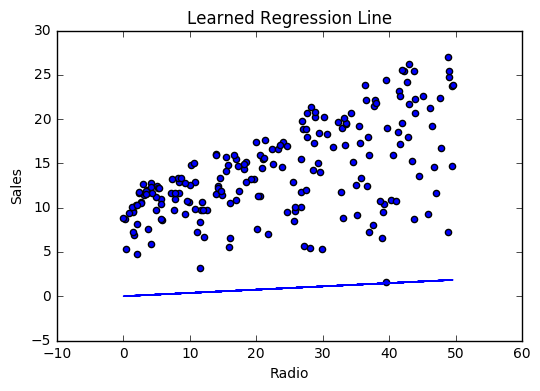
\includegraphics[width=0.9\linewidth]{fig/plot_simple_reg_1.png}
        \caption{ครั้งที่ 1}
        \label{fig:plot_simple_reg_1}
    \end{subfigure}
    \\
    \begin{subfigure}{0.8\textwidth}
        \centering
        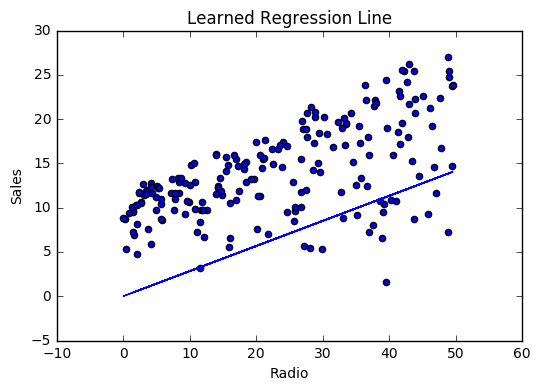
\includegraphics[width=0.9\linewidth]{fig/plot_simple_reg_2.png}
        \caption{ครั้งที่ 2}
        \label{fig:plot_simple_reg_2}
    \end{subfigure}
\end{figure}%
\begin{figure}[htbp]\ContinuedFloat
    \centering
    \begin{subfigure}{0.8\textwidth}
        \centering
        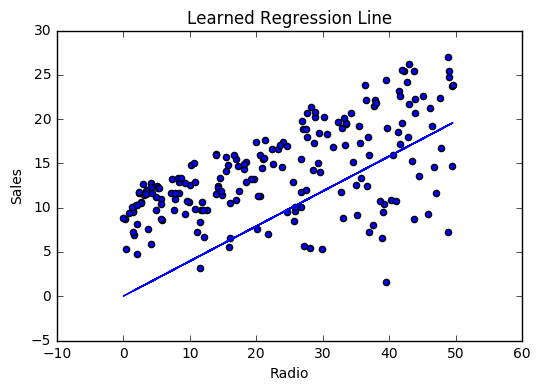
\includegraphics[width=0.9\linewidth]{fig/plot_simple_reg_3.png}
        \caption{ครั้งที่ 3}
        \label{fig:plot_simple_reg_3}
    \end{subfigure}
    \\
    \begin{subfigure}{0.8\textwidth}
        \centering
        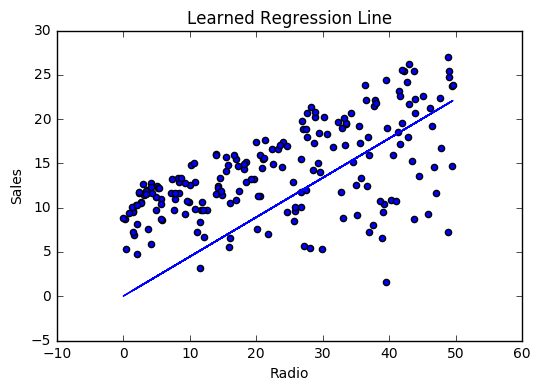
\includegraphics[width=0.9\linewidth]{fig/plot_simple_reg_4.png}
        \caption{ครั้งที่ 4}
        \label{fig:plot_simple_reg_4}
    \end{subfigure}
    \caption{การเปลี่ยนแปลงของเส้นตรงที่ถูกทาบ (Fitting) เข้ากับชุดข้อมูลอย่างง่าย}
    \label{fig:simple_reg_change}
\end{figure}

%--------------------------
\subsection{การถดถอยแบบหลายตัวแปร}
\label{ssec:multi_lin_res}
\idxth{การเรียนรู้แบบมีผู้สอน!การถดถอยแบบหลายตัวแปร}
\idxen{Supervised Learning!Multivariate Regression}
%--------------------------

สำหรับกรณีที่เรามีอินพุตหรือ Feature มากกว่าหนึ่งตัว เช่น ข้อมูลในตาราง \ref{tab:multi_reg_data} ด้านล่างที่เป็นการนำข้อมูลในตาราง 
\ref{tab:simple_reg_data} มาเพิ่มข้อมูลเงินที่ใช้ในการลงทุนสำหรับการโฆษณาทางสื่อโทรทัศน์และหนังสือพิมพ์เข้าไป (คอลัมน์ที่ 3 กับ 4) 

\begin{table}[htbp]
    \centering
    \caption{แสดงเงินที่ใช้ในการลงทุนการโฆษณาของบริษัทต่าง ๆ กับยอดขายรายปี}
    \label{tab:multi_reg_data}
    \begin{tabular}{lcccc}\toprule
    \textbf{บริษัท} &\textbf{วิทยุ} &\textbf{โทรทัศน์} &\textbf{หนังสือพิมพ์} &\textbf{ยอดขาย (ต่อหน่วย)} \\\midrule
    Amazon &37.8 &230.1 &69.1 &22.1 \\
    Google &39.3 &44.5 &23.1 &10.4 \\
    Facebook &45.9 &17.2 &34.7 &18.3 \\
    Apple &41.3 &151.5 &13.2 &18.5 \\
    \bottomrule
    \end{tabular}
\end{table}

\begin{figure}[htbp]
    \centering
    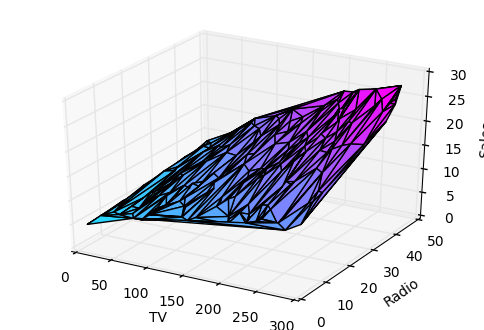
\includegraphics[width=0.8\linewidth]{fig/plot_multivar_reg.png}
    \caption{ความสัมพันธ์ของข้อมูลหลายตัวแปร (Multivariables Data)}
    \label{fig:multi_var_reg}
\end{figure}

โดยในกรณีที่ข้อมูลมีความซับซ้อนมากขึ้นแบบนี้ เราไม่สามารถใช้สมการเส้นตรงแบบง่าย ๆ ที่เราใช้ไปก่อนหน้านี้มาอธิบายความสัมพันธ์ระหว่าง 
Feature ได้ ดังนั้นเราจะต้องมีการกำหนด Loss Function ขึ้นมาใหม่ โดยตอนนี้เราจะต้องมีการกำหนดค่า Weight ขึ้นมา 3 ค่า นั่นคือจากที่%
เราเคยมีฟังก์ชัน $mx + b$ ก็จะกลายเป็นฟังก์ชัน $W_1 x_1 + W_2 x_2 + W_3 x_3$ โดยจะได้สมการ Loss Function ใหม่ดังนี้

\begin{equation}
    \text{MSE} = \frac{1}{2N} \sum_{i=1}^{n} (y_i - (W_1 x_1 + W_2 x_2 + W_3 x_3))^2
\end{equation}

สำหรับสมการที่เราจะมาใช้ในการหา Gradient ของกรณีนี้สามารถพิสูจน์ได้โดยใช้กฎลูกโซ่ (Chain Rule) เช่นเดียวกับกรณีก่อนหน้านี้

\begin{align}
    f'(W_1) = -x_1(y - (W_1 x_1 + W_2 x_2 + W_3 x_3)) \\
    f'(W_2) = -x_2(y - (W_1 x_1 + W_2 x_2 + W_3 x_3)) \\
    f'(W_3) = -x_3(y - (W_1 x_1 + W_2 x_2 + W_3 x_3))
\end{align}

%--------------------------
\section{การจำแนกประเภท}
\label{sec:classification}
\idxth{การเรียนรู้แบบมีผู้สอน!การจำแนกประเภท}
\idxen{Supervised Learning!Classification}
%--------------------------

ในหัวข้อนี้จะเป็นการศึกษาโจทย์ปัญหาแบบการจำแนกประเภท (Classification) ซึ่งก็คล้าย ๆ กับโจทย์แบบ Regression แต่ว่าจะต่างกันตรงที่ค่า
$y$ ที่เราต้องการทำนายนั้นจะมีความไม่ต่อเนื่อง (Discrete Data) ซึ่งจะตรงข้ามกับ Regression ที่ค่า $y$ จะมีความต่อเนื่อง (Continuous 
Data) โดยเริ่มต้นเราจะสนใจกรณี Classification แบบง่ายก่อน นั่นก็คือมีประเภทของข้อมูลที่เราจะจำแนกเพียงแค่ 2 ประเภท เรียกว่าโจทย์ปัญหา 
Binary Classification ซึ่งค่า $y$ จะมีค่าได้แค่ 0 กับ 1 เท่านั้น ซึ่งในภายหลังเราจึงค่อยมาพิจารณากรณีที่มีประเภทมากกว่า 2 ประเภท
(Multiple-class Case) 

สำหรับการระบุชื่อของประเภทหรือคลาส (Class) นั้น เราจะเรียกคลาส 0 ว่าเป็น Negative Class และเรียกคลาส 1 ว่า Positive Class
ซึ่งบ่อยครั้งเรามักจะเจอการใช้เครื่องหมาย - และ + แทนการเขียน 0 กับ 1 โดยที่เราจะกำหนดให้ $y^{i}$ คือ Label ของข้อมูลลำดับที่ $i$ 
สำหรับตัวอย่างการฝึกสอน

%--------------------------
\section{การถดถอยแบบโลจิสติค}
\label{sec:logis_regress}
\idxth{การเรียนรู้แบบมีผู้สอน!การถดถอยแบบโลจิสติค}
\idxen{Supervised Learning!Logistic Regression}
%--------------------------

การวิเคราะห์การถดถอยโลจิสติค (Logistic Regression) เป็นการวิเคราะห์ที่มีเป้าหมายเพื่อประมาณค่าหรือทํานายเหตุการณ์ที่สนใจว่าจะเกิดหรือ%
ไม่เกิดเหตุการณ์นั้นภายใต้อิทธิพลของตัวปัจจัยโดยอาศัยฟังก์ชันโลจิสติค (Logistic Function) ที่สร้างขึ้นจากชุดตัวแปรทำนายที่เป็นตัวแปรที่มีข้อมูล%
อยู่ในระดับช่วงเป็นอย่างน้อย โดยที่ระหว่างตัวแปรทำนายจะต้องมีความสัมพันธ์กันต่ำและในการวิเคราะห์จะต้องใช้ขนาดตัวแปรทำนายไม่ต่ำกว่า 30 
ตัวแปร Logistic Regression จัดเป็นเครื่องมือวิเคราะห์ข้อมูลในการศึกษาวิจัยที่มีวัตถุประสงค์เพื่อทํานายเหตุการณ์หรือประเมินความเสี่ยง (เช่น 
\enquote{เสี่ยง} หรือ \enquote{ไม่เสี่ยง}) จึงมีการประยุกต์ใช้ในงานวิจัยหลากหลายสาขา ทั้งสาขาทางการแพทย์ วิศวกรรมศาสตร์ นิเวศวิทยา 
เศรษฐศาสตร์ และสังคมศาสตร์
\idxboth{การถดถอยโลจิสติค}{Logistic Regression}
\idxboth{ฟังก์ชันโลจิสติค}{Logistic Function} 

นอกจากการทำนายการเกิดเหตุการณ์ที่สนใจว่าเกิด (0) หรือไม่เกิด (1) ได้แล้ว Logistic Regression ยังสามารถทำนายค่าความน่าจะเป็นของ%
เหตุการณ์ได้ด้วย (ค่าระหว่าง 0 กับ 1) จริง ๆ แล้วเทคนิค Logistic Regression นั้นคล้ายกับ Linear Regression มาก โดยทั้งสองเทคนิค%
นี้ต่างกันตรงที่การนำไปใช้งาน โดยเราใช้ Linear Regression สำหรับการแก้ปัญหาการถดถอยแต่ Logistic Regression สำหรับการแก้ปัญหา%
การแยกคลาสหรือจัดกลุ่มของข้อมูล

\begin{figure}[htbp]
    \centering
    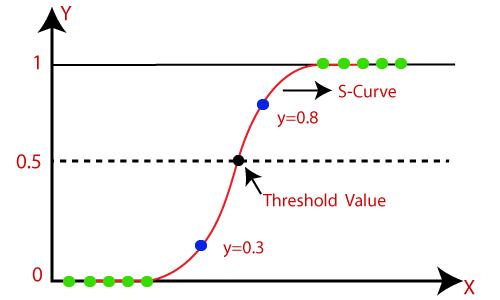
\includegraphics[width=0.8\linewidth]{fig/s_curve_logistic_func.png}
    \caption{Logistic Function หรือ Sigmoid Function}
    \label{fig:s_curve_logistic}
\end{figure}

การทำ Losgistic Regression นั้นเราไม่ได้ทำการ Fit เส้น Regression กับข้อมูลแต่จะเป็นการ Fit กับ Logistic Function (ภาพที่ 
\ref{fig:s_curve_logistic}) แทนซึ่งจะเป็นตัวที่ทำนายค่าออกมา โดย Logistic Function ที่เราใช้นั้นจริง ๆ แล้วก็คือเส้นโค้งตัว S หรือ
Sigmoid Function นั่นเอง โดยมีนิยามทางคณิตศาสตร์ดังต่อไปนี้
\idxen{Supervised Learning!Logistic Regression!Sigmoid Function}

\begin{equation}\label{eq:logistic_func}
    f(x) = \frac{L}{1 + e^{-k(x-x_0)}}
\end{equation}

\noindent สำหรับกรณีที่กำหนดให้ $k = 1$, $x_{0} = 0$, และ $L = 1$ เราจะได้สมการดังต่อไปนี้

\begin{align}\label{eq:std_logis_func}
    f(x) &= \frac{1}{1 + e^{-x}} \nonumber \\
    &= \frac{e^x}{e^x + 1} \nonumber \\
    &= \frac12 + \frac12 \tanh\left(\frac{x}{2}\right)
\end{align}

\noindent ซึ่งเราเรียกสมการที่ \ref{eq:std_logis_func} นี้ว่าฟังก์ชันโลจิสติคมาตรฐาน (Standard Logistic Function)
\idxth{การเรียนรู้แบบมีผู้สอน!การถดถอยแบบโลจิสติค!ฟังก์ชันโลจิสติคมาตรฐาน}
\idxen{Supervised Learning!Logistic Regression!Standard Logistic Function}

โดยเทคนิคนี้ถูกนำมาใช้เยอะมากใน ML เพราะว่ามีความสามารถในการทำนายค่าความน่าจะเป็นและแยกข้อมูลโดยใช้ชุดข้อมูลที่มีความต่อเนื่องหรือ%
แบบไม่ต่อเนื่องก็ได้ หนังสือบางเล่มหรือบทความวิจัยบางฉบับเรียก Logistic Regression ว่า Maximum-entropy Classification (MaxEnt) 
หรือ Log-linear Classifier เพราะว่าถูกนำมาใช้กับโจทย์ปัญหา Classification มากกว่า Regression ตามที่ได้อธิบายไว้

โค้ดด้านล่างคือตัวอย่างการเรียกใช้ฟังก์ชัน \inlinehighlight{LogisticRegression} ของไลบรารี่ Scikit-Learn สำหรับการฝึกสอนโมเดล%
ด้วย Logistic Regression โดยใช้ข้อมูลตัวอย่างที่สมมติขึ้นมา

\begin{lstlisting}[style=MyPython]
import numpy as np
from sklearn.linear_model import LogisticRegression

# Create dataset
x = np.arange(10).reshape(-1, 1)
y = np.array([0, 0, 0, 0, 1, 1, 1, 1, 1, 1])

# Create a logistic regression model
model = LogisticRegression(solver='liblinear', random_state=0)

# Train the model
model.fit(x, y)

# Get results
model.classes_
# Output
array([0, 1])
model.intercept_
# Output
array([-1.04608067])
model.coef_
# Output
array([[0.51491375]])
\end{lstlisting}

\vspace{1em}

เราสามารถแสดงเมทริกซ์ของค่าความน่าจะเป็น (Probability Matrix) ของข้อมูลแต่ละตัวได้ด้วย ดังนี้

\begin{lstlisting}[style=MyPython]
model.predict_proba(x)
# Output
array([[0.74002157, 0.25997843],
       [0.62975524, 0.37024476],
       [0.5040632 , 0.4959368 ],
       [0.37785549, 0.62214451],
       [0.26628093, 0.73371907],
       [0.17821501, 0.82178499],
       [0.11472079, 0.88527921],
       [0.07186982, 0.92813018],
       [0.04422513, 0.95577487],
       [0.02690569, 0.97309431]])
\end{lstlisting}

%--------------------------
\section{เครื่องเวกเตอร์ค้ำยัน}
\label{sec:svm}
\idxth{การเรียนรู้แบบมีผู้สอน!เครื่องเวกเตอร์ค้ำยัน}
\idxen{Supervised Learning!Support Vector Machine}
%--------------------------

เครื่องเวกเตอร์ค้ำยัน (Support Vector Machine หรือ SVM) เป็นวิธีเคอร์เนลแบบหนึ่งที่มีความคล้ายกับ GPR หรือ KRR เป็นอย่างมาก โดย SVM 
จะทำการทำนายค่าโดยทำการเปรียบเทียบข้อมูลใหม่กับข้อมูลอ้างอิงด้วยฟังก์ชัน $k(x_{i},x_{j})$ และคำนวณค่าความเหมือน (Similarity) 
ระหว่างจุดสองจุด ซึ่งเราเรียกสิ่งนี้ว่าเคอร์เนล (Kernel) โดยความซับซ้อนของวิธีนี้นั้นไม่มีกฎเกณฑ์ที่แน่นอนในการกำหนด (Arbitrarily)
ดังนั้นเราจะต้องทำการปรับ Hyperparameters เพื่อให้มีความเหมาะสมและสามารถควบคุมความซับซ้อนของวิธี SVM ซึ่งเราเรียกวิธีการปรับนี้ว่า 
Regularization เพื่อทำการหลีกเลี่ยงปัญหา Overfit นั่นเอง ผู้อ่านสามารถศึกษาเคอร์เนลเพิ่มเติมได้ในหัวข้อที่ \ref{sec:kernel}
\idxboth{การทำให้ถูกต้อง}{Regularization}

\begin{figure}[htbp]
    \centering
    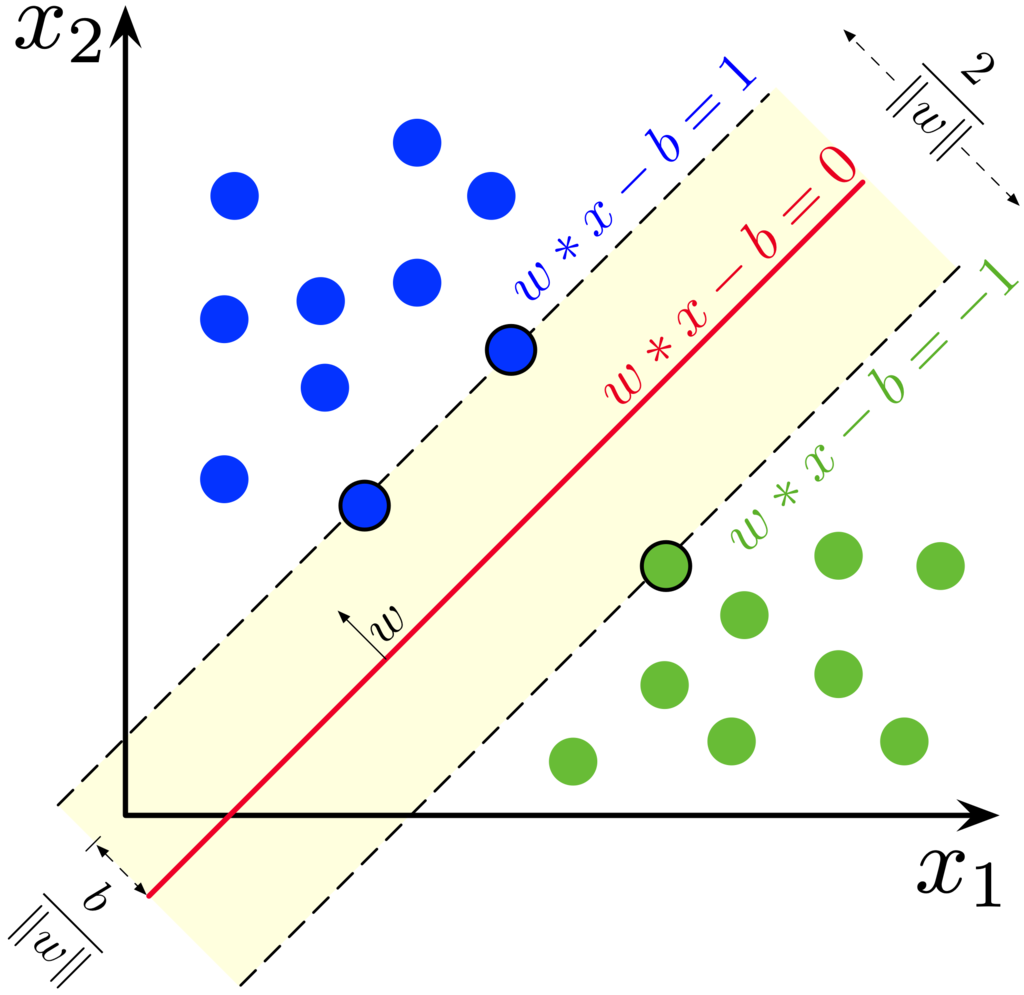
\includegraphics[width=0.65\linewidth]{fig/svm.png}
    \caption{Maximum Margin Hyperplan และ Margi สำหรับการฝึกสอนโมเดลของชุดข้อมูลตัวอย่างที่มี 2 คลาสด้วย Support Vector 
    Machine (เครดิตภาพ: \url{https://en.wikipedia.org/wiki/Support_vector_machine})}
    \label{fig:svm_margin}
\end{figure}

ภาพที่ \ref{fig:svm_margin} แสดงชุดข้อมูลตัวอย่างที่มี 2 คลาส (สีน้ำเงินกับสีเขียว) โดยมีระนาบระยะห่างที่มากที่สุด (Maximum Margin 
Hyperplan หรือ MMH) เป็นตัวแบ่งข้อมูลซึ่งอ้างอิงโดยจุดข้อมูลที่อยู่ใกล้กับ Hyperplan ซึ่งจุดข้อมูลเหล่านี้มีชื่อเรียกว่าเวกเตอร์ค้ำยัน (Support 
Vector) โดยเราคำนวณ Support Vector จากช่องว่าง (Margin) ระหว่างคลาสทั้ง 2 คลาสโดยใช้ระยะห่างที่น้อยที่สุด ดังนั้นเป้าหมายของการ%
ฝึกสอนโมเดลด้วย SVM ก็คือการหา Hyperplan ที่สามารถแบ่งข้อมูลทั้ง 2 คลาสออกจากกันได้ดีที่สุด
\idxen{Supervised Learning!Support Vector Machine!Hyperplane}
\idxen{Supervised Learning!Support Vector Machine!Margin}

โค้ดด้านล่างคือตัวอย่างการเรียกใช้ฟังก์ชัน \inlinehighlight{svm} ของไลบรารี่ Scikit-Learn สำหรับการฝึกสอนโมเดลด้วย SVM โดยใช้%
ข้อมูลตัวอย่างที่สมมติขึ้นมา

\begin{lstlisting}[style=MyPython]
import numpy as np
from sklearn import svm

# Create dataset
x = np.arange(10).reshape(-1, 1)
y = np.array([0, 0, 0, 0, 1, 1, 1, 1, 1, 1])
x_test = x + 1.2

# Create a SVM classifier using linear kernel
clf = svm.SVC(kernel='linear')

# Train the model
clf.fit(x, y)

# Predict the response for test dataset
clf.predict(x_test)
# Output
array([0, 0, 0, 1, 1, 1, 1, 1, 1, 1])
\end{lstlisting}

%--------------------------
\section{เทคนิคการเรียนรู้แบบมีผู้สอนแบบอื่น ๆ}
\label{sec:other_ml}
\idxth{เทคนิคการเรียนรู้แบบผู้มีสอน}
\idxth{เทคนิคการเรียนรู้ของเครื่อง}
\idxen{Machine Learning Techniques}
\idxen{Unsupervised Machine Learning Techniques}
%--------------------------

%--------------------------
\subsection{Partial Least Squares (PLS)}
\label{ssec:pls}
\idxth{เทคนิคการเรียนรู้ของเครื่อง!วิธีกำลังสองน้อยที่สุดบางส่วน}
\idxen{Machine Learning Techniques!Partial Least Squares}
%--------------------------

วิธีกำลังสองน้อยที่สุดบางส่วน (Partial Least Squares หรือ PLS) เป็นวิธีเชิงสถิติที่ใช้สำหรับการวิเคราะห์หลายตัวแปรเพื่อสร้างตัวแบบ%
ความสัมพันธ์ระหว่างกลุ่มของตัวแปรทำนาย (Predictor Variable) โดยอาศัยตัวแปรแฝง (Latent variable) ซึ่งเทคนิคนี้มีความคล้ายกับ 
Principle Component Analysis (PCA) ซึ่งจะเป็นการลดจำนวนมิติของข้อมูล\autocite{wold1984} ในช่วงยุคเริ่มต้นที่มีการใช้ปัญญาประดิษฐ์%
ในงานด้านเคมีนั้น เทคนิคนี้ได้ถูกนำมาใช้อย่างแพร่หลาย เช่น นำมาใช้สำหรับการระบุ Vibrational Bands สำหรับ Vibrational Spectra 
และนำผลที่ได้มาเปรียบเทียบกับค่าการทำนายที่ได้จากวิธีอื่น เช่น ANN และ PCA-ANN

%--------------------------
\subsection{Gaussian Process Regression (GPR)}
\label{ssec:gpr}
\idxth{เทคนิคการเรียนรู้ของเครื่อง!การถดถอยของกระบวนการเกาส์เซียน}
\idxen{Machine Learning Techniques!Gaussian Process Regression}
%--------------------------

การถดถอยของกระบวนการเกาส์เซียน (Gaussian Process Regression หรือ GPR) เป็นวิธีการถดถอยของเบส์แบบหนึ่งโดยใช้ Kernel Function 
ที่สามารถบ่งบอกหรือแสดงค่าความแปรปรวน (Covariance) ในขั้นตอน Gaussian Process ได้\autocite{rasmussen2005} โดย GPR 
จะทำการสร้างโมเดลแบบ Non-parametric และสามารถคำนวณค่าความเชื่อมั่น (Confidence Intervals) ไปพร้อม ๆ กับการทำนาย 
รายละเอียดเพิ่มเติมของ GPR สามารถศึกษาได้ในหัวข้อ \ref{sec:gaussian_process}

%--------------------------
\subsection{Random Forest}
\label{ssec:rs}
\idxth{เทคนิคการเรียนรู้ของเครื่อง!เครื่องเวกเตอร์ค้ำยัน}
\idxen{Machine Learning Techniques!Random Forest}
%--------------------------

การสุ่มป่าไม้ (Random Forest หรือ RF) เป็นวิธีหนึ่งในกลุ่มของโมเดลที่เรียกว่าการเรียนรู้แบบกลุ่มก้อน (Ensemble Learning) ที่มีหลักการคือ%
การฝึกสอนโมเดลที่เหมือนกันหลาย ๆ ครั้ง (Multitude) บนข้อมูลชุดเดียวกัน โดยแต่ละครั้งของการเทรนจะเลือกส่วนของข้อมูลที่ฝึกสอนไม่เหมือนกัน 
แล้วนำการตัดสินใจของโมเดลเหล่านั้นมาโหวตเลือกกันว่า Class ไหนถูกเลือกมากที่สุด\autocite{breiman2001,quinlan1986}

ตัวอย่างการเขียนโค้ดโมเดล Random Forest สำหรับการทำ Regression 

\begin{lstlisting}[style=MyPython]
from sklearn.ensemble import RandomForestRegressor
from sklearn.datasets import make_regression

X, y = make_regression(n_features=4, n_informative=2,
                       random_state=0, shuffle=False)
regr = RandomForestRegressor(max_depth=2, random_state=0)
regr.fit(X, y)

print(regr.predict([[0, 0, 0, 0]]))
# Output
[-8.32987858]
\end{lstlisting}

\vspace{1em}

ตัวอย่างการเขียนโค้ดโมเดล Random Forest สำหรับการทำ Classification 

\begin{lstlisting}[style=MyPython]
from sklearn.ensemble import RandomForestClassifier
from sklearn.datasets import make_classification

X, y = make_classification(n_samples=1000, n_features=4,
                           n_informative=2, n_redundant=0,
                           random_state=0, shuffle=False)
clf = RandomForestClassifier(max_depth=2, random_state=0)
clf.fit(X, y)

print(clf.predict([[0, 0, 0, 0]]))
# Output
[1]
\end{lstlisting}

%--------------------------
\subsection{Artificial Neural Network}
\label{ssec:ann}
\idxth{เทคนิคการเรียนรู้ของเครื่อง!โครงข่ายประสาทเทียมประดิษฐ์}
\idxen{Machine Learning Techniques!Artificial Neural Network}
%--------------------------

โครงข่ายประสาทเทียมประดิษฐ์ (Artificial Neural Network หรือ ANN) หรือเรียกว่าโครงข่ายประสาทเทียม (Neural Network หรือ 
Neural Net) เป็นอัลกอริทึมรูปแบบหนึ่งที่เลียนแบบการทำงานของสมองมนุษย์ โดยทำการสร้างโมเดลเรียนรู้ที่ประกอบไปด้วยชั้นเรียนรู้ระหว่างกลาง 
(Hidden Layer) และหน่วยย่อยที่เกิดการเรียนรู้ (Node หรือ Artificial Neuron หรือ Unit)

\begin{figure}[htbp]
    \centering
    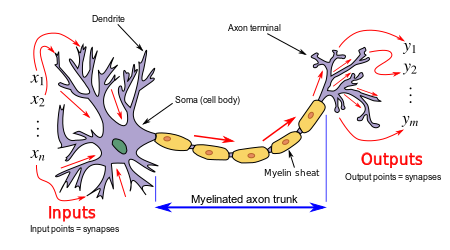
\includegraphics[width=0.9\linewidth]{fig/neuron.png}
    \caption{การรับส่งข้อมูลภายในเซลล์ประสาท}
    \label{fig:neuron}
\end{figure}

จริง ๆ แล้ว Neural Network ก็คือการจำลองสมองมนุษย์โดยพยายามสร้างองค์ประกอบต่าง ๆ ให้มีความคล้ายกันให้มากที่สุด เช่น ในสมองมี%
เซลล์ประสาท (Neurons) และจุดประสานประสาท (Synapses) แต่ละเซลล์ประสาทประกอบด้วยปลายในการรับกระแสประสาทเรียกว่า 
\enquote{เดนไดรท์} (Dendrite) ซึ่งเป็นอินพุตและปลายในการส่งกระแสประสาทเรียกว่าแอคซอน (Axon) ซึ่งเปรียบเหมือนเป็นเอาต์พุตของเซลล์

โดยโมเดล Neural Network ที่มีการนำไปใช้มากที่สุดคือเครือข่ายประสาทแบบป้อนไปหน้า (Feed-forward Network) และโมเดล Neural Network 
ยังสามารถแบ่งออกได้เป็นหลายประเภท ดังนี้

\begin{itemize}
    \item เพอร์เซ็ปตรอนชั้นเดียว (Single-layer Perceptron)
    
    \item เพอร์เซ็ปตรอนหลายชั้น (Multi-layer Perceptron)
    
    \item โครงข่ายแบบวนซ้ำ (Recurrent Neural Network)
    
    \item แผนผังจัดระเบียบเองได้ (Self-organizing Map)
    
    \item เครื่องจักรโบลทซ์แมน (Boltzmann Machine)
    
    \item กลไกแบบคณะกรรมการ (Committee of Machines)
    
    \item โครงข่ายความสัมพันธ์ (Associative Neural Network)
    
    \item โครงข่ายกึ่งสำเร็จรูป (Instantaneously Trained Networks)
    
    \item โครงข่ายแบบยิงกระตุ้น (Spiking Neural Networks) 
\end{itemize}

โดยในหนังสือเล่มนี้จะอธิบายเฉพาะ Neural Network แบบเพอร์เซ็ปตรอนชั้นเดียวและเพอร์เซ็ปตรอนหลายชั้น (บทที่ \ref{ch:deep_learning}) 
สำหรับผู้อ่านที่สนใจศึกษารายละเอียดของ Neural Network ประเภทอื่น ๆ นั้นสามารถศึกษาได้จากหนังสือเฉพาะทางด้าน Neural Network เช่น 
\enquote{Deep Learning} เขียนโดย Ian Goodfellow, Yoshua Bengio และ Aaron Courville\autocite{Goodfellow-et-al-2016} 
รายละเอียดเพิ่มเติมดูได้ที่เว็บไซต์ \url{https://www.deeplearningbook.org}
